\documentclass[a4paper]{article}
\usepackage[frenchb]{babel}
\usepackage[utf8]{inputenc}
%\usepackage[T1]{fontenc}
%\usepackage{lmodern}
\usepackage{amsmath}
%\usepackage{tikz}
%\usepackage{cite}
\usepackage{hyperref}
%\usepackage{fancyvrb}
%\usepackage{bm}
%\usepackage{pxfonts}
\usepackage{verbatim}
\usepackage{a4wide}
\usepackage{graphicx}

\hypersetup{
  backref=true, %permet d'ajouter des liens dans...
  pagebackref=true,%...les bibliographies
  hyperindex=true, %ajoute des liens dans les index
  colorlinks=true, %colorise les liens
  breaklinks=true, %permet le retour a la ligne dans les liens trop longs
  urlcolor=blue,  %couleur des hyperliens (blue pour la version web)
  linkcolor=blue, %couleur des liens internes (blue pour la version web)
  citecolor=blue, %couleur des citation (green pour la version web)
  bookmarks=true,  %cree des signets pour Acrobat
  bookmarksopen=true, %affiche completement les signets Acrobat
  %%%%%%%%%%%%%%%%% HYPER TITLE %%%%%%%%%%%%%%%%%%%%%%%%%%
  pdfsubject={Rapport} %document sous Acrobat.
}

% Alter some LaTeX defaults for better treatment of figures:
% See p.105 of "TeX Unbound" for suggested values.
% See pp. 199-200 of Lamport's "LaTeX" book for details.
% General parameters, for ALL pages:

%\renewcommand{\topfraction}{0.9}  % max fraction of floats at top
%\renewcommand{\bottomfraction}{0.8} % max fraction of floats at bottom


% Parameters for TEXT pages (not float pages):

%\setcounter{topnumber}{2}
%\setcounter{bottomnumber}{2}
%\setcounter{totalnumber}{4}     % 2 may work better
%\setcounter{dbltopnumber}{2}    % for 2-column pages

%\renewcommand{\dbltopfraction}{0.9} % fit big float above 2-col. text
%\renewcommand{\textfraction}{0.07}  % allow minimal text w. figs
% Parameters for FLOAT pages (not text pages):
%\renewcommand{\floatpagefraction}{0.7}  % require fuller float pages
% N.B.: floatpagefraction MUST be less than topfraction !!
%\renewcommand{\dblfloatpagefraction}{0.7} % require fuller float pages

% remember to use [htp] or [htpb] for placement


\newcommand{\FIXME}{\textcolor{red}{FIXME}}
%\newcommand{\TODO}[1]{(\textcolor{red}{TODO} #1)}
\newcommand{\TODO}[1]{}
\newcommand{\LANG}{{\sc Heptagon}}
\newcommand{\lucy}{{\sc Lucid Synchrone}}
\newcommand{\lustre}{{\sc Lustre}}
\newcommand{\scade}{{\sc Scade}}
\newcommand{\scadesix}{{\sc Scade~6}}
\newcommand{\minils}{{\sc MiniLS}}
\newcommand{\heptagon}{{\sc Heptagon}}
\newcommand{\obc}{{\sc Obc}}
\newcommand{\minivhdl}{{\sc MiniVHDL}}
\newcommand{\vhdl}{{\sc Vhdl}}


\newcommand{\bold}[1]{\textbf{#1}}
\newcommand{\p}[0]{\; \vert \;}
\newcommand{\rst}[1]{Rst(#1)}
\newcommand{\rstnd}[1]{RstNode(#1)}
% \newcommand{\rst}[1]{\llbracket #1 \rrbracket^{rst}}
\newcommand{\tvh}[2]{\llbracket #2 \rrbracket^{vhdl\ #1}}
\newcommand{\guardb}[1]{\llbracket #1 \rrbracket^{guard}}
\newcommand{\guard}[2]{\mbox{if } \guardb{#1} \mbox{ then } #2 \mbox{ else }
  \emptyset}
\newcommand{\mybox}[1]{\mbox{\tt{#1}}}
\newcommand{\bl}[0]{\hspace{0.45cm}}
\newcommand{\ind}[0]{\hspace{0.5cm}}
\newcommand{\Cons}[0]{\; \mathbf{::} \;}
\newcommand{\Coloneqq}[0]{::=}
\newcommand{\coloneqq}[0]{::=}
%% Syntaxe MiniLS

\newcommand{\Node}[4]{\mybox{node} \; f(#1) = #2 \; \mybox{with var} \
  #3 \; \mybox{in} \; #4}
\newcommand{\Op}[2]{\mybox{\bf{op}}(#1,\dots,#2)}
\newcommand{\Fby}[2]{#1 \, \mybox{fby}^{ck} \, #2}
\newcommand{\Pre}[1]{\mybox{pre}^{ck} \, #1}
\newcommand{\Every}[4]{#1^{ck}(#2,\dots,#3) \, \mybox{every} \, #4}
\newcommand{\App}[2]{#1^{ck}(#2)}
\newcommand{\If}[3]{\mybox{if} \; #1 \; \mybox{then} \; #2 \; \mybox{else} \; #3}
\newcommand{\When}[3]{#1 \; \mybox{when} \; #2(#3)}
\newcommand{\Merge}[5]{\mybox{merge} \; #1 \; (#2 \Rightarrow #3) \; \dots \; \
  (#4 \Rightarrow #5)}
\newcommand{\Merges}[5]{\mybox{merge} \; #1 \; (#2 \Rightarrow #3) \; \
  (#4 \Rightarrow #5)}
\newcommand{\Base}[0]{\mybox{base}}
\newcommand{\On}[3]{#1 \; \mybox{on} \; #2 (#3)}
\newcommand{\Map}[3]{\mathtt{map} \; #1\; n\; (#2,\dots,#3)}
\newcommand{\Fold}[3]{\mathtt{fold} \; #1\; n\; (#2,\dots,#3)}
\newcommand{\Mapfold}[3]{\mathtt{mapfold} \; #1\; n\; (#2,\dots,#3)}

%% Syntaxe VHDL

\newcommand{\Component}[6]{\mybox{component} \; #1 \; \mybox{port} \; #2 \; \
  \mybox{with} \; \mybox{sig} \; #3 \; \mybox{and} \; \mybox{var} \; #4 \; \\
  \mybox{and} \; \mybox{subcomponents} \; #5 \; \mybox{in} \; #6}

\newcommand{\Assign}[2]{#1 \Leftarrow #2}
\newcommand{\Affect}[2]{#1 \coloneqq #2}
\newcommand{\Case}[5]{\mybox{case} \; #1 \; \mybox{of} \; (#2 \Rightarrow #3) \
  \dots (#4 \Rightarrow #5)}

\title{Traduction SCADE/Lustre vers VHDL~\thanks{Rapport d'étude dans
    le cadre du projet GENCOD.}}  \author{Adrien Guatto et Marc Pouzet
  \\ LRI~\thanks{Marc Pouzet est maintenant professeur à l'Université
    Pierre et Marie Curie et rattaché à l'École normale
    supérieure. Adrien Guatto, étudiant de l'Université Pierre et
    Marie Curie, a effectué son stage dans le cadre du projet.}}
\date{31 août 2010}

\begin{document}

\maketitle

\section{Introduction}
Ce document présente le problème de la compilation d'un langage
synchrone tel que \scade{} vers un langage pour le matériel et les
circuits tel que \vhdl. Nous décrivons le problème posé, les
principales solutions envisagées et la solution proposée par le LRI.

Ce travail s'est appuyé sur la réalisation d'un prototype d'étude,
appelé \LANG{}. Il s'agit d'un compilateur produisant à la fois du
code séquentiel (ici, principalement C et Java) et du code \vhdl{} à
partir d'un programme synchrone. Le langage d'entrée est un
sous-ensemble de \scadesix{} et en reprend les principales
constructions: équations data-flow, automates hiérarchiques et
tableaux. Son compilateur est organisé de manière similaire au
compilateur KCG de \scade{} développé par
Esterel-Technologies~\footnote{Pour être complet, \LANG{} est un
  sous-ensemble du langage \lucy~\cite{lucy:manual06} dont plusieurs
  traits sont intégrés à \scadesix. Nous aurions donc pu
  réaliser un prototype d'étude à partir de \lucy. Le
  langage étant plus riche (ordre supérieur, inférence de type,
  polymorphisme, etc.), cela nécessitait de résoudre des problèmes peu
  pertinents pour le projet GENCOD. D'où le choix de considérer un
  langage simplifié.}.  Le prototype
\LANG{} a été mis a la disposition des partenaires du projet GENCOD.

\subsection{Compilation de SCADE/Lustre vers VHDL}

\begin{figure}[t]
\begin{center}
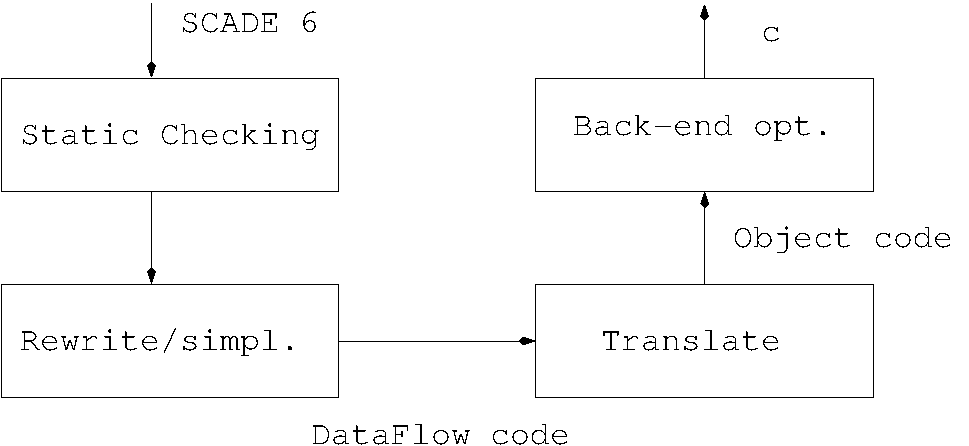
\includegraphics[height=4cm]{Fig/compil-scade}
\end{center}
\caption{Organisation générale du compilateur de SCADE~\label{organisation-scade}}
\end{figure}

Rappelons l'organisation générale du compilateur KCG
(Figure~\ref{organisation-scade}).  La compilation d'un programme se
déroule en quatre grandes étapes: 1/ une phase d'analyse statique
(typage~\cite{lucy:emsoft03}, calcul d'horloges~\cite{lucy:emsoft04},
analyse de causalité et analyse d'initialisation~\cite{lucy:sttt04});
2/ une phase comportant une succession de réécritures produisant à la
fin un code data-flow avec horloges; cette étape élimine les
principales structures de contrôle (automates, conditions
d'activations) en produisant des équations ``gardées''; 3/ une phase
de compilation du code data-flow vers du code impératif séquentiel
(object code); chaque noeud \scade{} est représenté par une fonction
de transition; 4/ une phase d'optimisation appliquée au code
séquentiel (élimination des copies, propagation de constantes,
etc.). Au préalable à cette phase, les modules sont expansés et le
code polymorphe est spécialisé. Ces deux étapes préliminaires ne sont
pas décrites ici.

Au regard de cette organisation, il y a deux points d'entrées naturels
pour produire du code \vhdl{}:
\begin{enumerate}
\item à partir du code intermédiaire data-flow avec horloges, après
  élimination des structures de contrôle (e.g., automates, conditions
  d'activation);
\item
à partir du code final généré par le compilateur (dans le cas de KCG, le
code C).
\end{enumerate}

Remarquons que le code intermédiaire data-flow est déjà un point d'entrée pour les
outils de vérification formelle utilisés dans le compilateur KCG (tels que
le plug-in de Prover Technology): la vérification d'une propriété (programmée
en \scade) est obtenue par traduction préalable vers le format data-flow,
format qui sert de passerelle vers l'outil Prover.

\subsection{Génération de VHDL à partir d'équations data-flow gardées}
Les deux solutions décrites ci-dessus ont été retenues dans le projet
GENCOD. La société GeenSoft a réalisé un compilateur à partir du code
C généré par KCG. Nous décrivons ici l'autre solution où le code
\vhdl{} est produit directement à partir des équations data-flow. Pour cela,
nous décrivons formellement chacune des étapes de traduction, dans une
perspective d'intégration dans une chaîne de compilation certifiée.

L'utilisation de Lustre pour la génération de matériel a été envisagée
très tôt (thèse de Frédéric Rocheteau~\cite{lustre:rocheteau91}). Signalons
également que \lustre{} est utilisé dans plusieurs enseignements de
matériel~\cite{lustre:amblard05}.

\subsubsection{Un mot sur la traduction de C vers VHDL}
L'intérêt principal de produire du code \vhdl{} à partir du code C généré par KCG est
de ne pas toucher au compilateur existant, déjà qualifié. À condition
de qualifier le générateur de code C vers \vhdl{} et de fournir les
informations de retour au source (tra\c{c}abilité), on peut envisager de disposer 
d'une chaîne qualifiée. Discutons ici des points délicats de cette solution.

La compilation de \scade{} est modulaire: un noeud \texttt{counter}
est traduit vers deux fonctions
C dont l'interface est schématiquement:

\begin{verbatim}
/* counter.c */
int counter_step(int counter_res, int counter_tick, counter_mem* self) { ... }

void counter_init(counter_mem* self)
  { self->counter_t1 = 0;
    self->counter_t2 = 0; }
\end{verbatim}
où:
\begin{verbatim}
typedef struct { 
  int counter_t1; 
  int counter_t2; }
counter_mem;
\end{verbatim}
\texttt{counter\_step} est la fonction de transition qui prend
en entrée un argument supplémentaire représentant son état interne. L'exécution
d'un pas produit une sortie et met à jour l'état interne (par effet de bord).
La fonction \texttt{counter\_init} permet d'initialiser l'état interne.

Le corps de ces deux fonctions est formé d'affectations de variables
locales où de l'état (ici \texttt{self}) ainsi que de structures de
contrôle (conditionnelles, construction ``switch'' et boucles ``for''
où d'appel à d'autres fonctions de transition). La génération de code
\vhdl{} suit le schéma suivant:

\begin{enumerate}
\item Une affectation de variable locale est traduite par une équation
  \vhdl{} sur une variable locale. E.g., \texttt{$x$ = $e$} est traduit
  schématiquement en une instruction \vhdl{} \texttt{$x$ := $e$}.  Il faut
  cependant être très attentif à ce que \verb-x- ne génère pas de
  registre.  Ce point est assez délicat puisque, en particulier lors
  de la traduction de \texttt{if $cond$ \{ $x$ = $exp$; \}}. Il
  correspond à la définition d'un flot dont l'horloge est
  $cond$. Parce que sa définition est partielle (la valeur de $x$ est
  indéfinie lorsque $cond$ est faux, sa traduction en \vhdl{} va conduire
  le synthétiseur à allouer un registre pour $x$, ce qui est à la fois
  inutile et inefficace.  Dans le cas où le programme en entrée n'a
  pas d'effets de bord, la sémantique de \scade{} garantit que ce
  programme est équivalent à l'affectation simple $x$ = $exp$.
\item Une affectation de variable d'état \texttt{self->$t$ =
    $exp$} doit être traduite vers une instruction de la forme
  \texttt{$t$ <= $exp$}. Cette affectation doit cependant être exécutée
  conditionnellement. Il faut donc retrouver, dans le code C,
  la condition booléenne d'activation de la mise à jour de
  l'état \texttt{self->$t$}.
\item La compilation des itérateurs (et plus largement des opérations de
manipulation des tableaux) est également délicate. Une équation de la forme:
\begin{verbatim}
t1 = map not <<10>>(t0)
\end{verbatim}
où \verb-t1- et \verb-t0- sont deux tableaux de taille 10 de valeurs
booléennes. Le code impératif produit le compilateur de \scade{} a
la forme suivante~\footnote{Nous donnons ici la sortie produite par le
  compilateur de \heptagon.}.
\begin{verbatim}
for (i = 0; i < 10; i++) {
  t1[i] = !t0[i]; }
\end{verbatim}
Or, le langage \vhdl{} dispose d'opérateurs agissant directement sur les
tableaux de bits (e.g., non logique, et logique). La bonne traduction
de la première équation est donc:
\begin{verbatim}
t1 := not t0;
\end{verbatim}
La génération de ce code, si elle est triviale à partir du code format data-flow,
parait délicate à partir du code impératif traduit par KCG.
\end{enumerate}

Retenons ici qu'une information précieuse pour la génération
de code \vhdl{} a été perdue durant la compilation vers du code séquentiel et
doit donc être reconstruite. Nous identifions trois autres
difficultés.
\begin{itemize}
\item La nécessité de certification demande d'instrumenter le
  compilateur KCG avec des informations donnant la tra\c{c}abilité (lien
  entre les noms de variables produites et les noms dans le code
  source, en particulier).
\item Certaines optimisations pertinentes lorsque l'on génère du code
  séquentiel, peuvent ne pas être utiles, voire pénalisantes, pour une
  compilation vers \vhdl{}. C'est le cas de l'optimisation des structures
  de contrôle ou de la compilation des boucles (cf. discussion
  ci-dessus, conduisant à générer trop de registres).
\item Il est nécessaire de restreindre le périmètre du compilateur C
  vers \vhdl{}: on ne réalise pas un compilateur capable de traduire tout
  code C vers \vhdl{} mais plutôt un compilateur adapté au code C produit
  par KCG et prenant en compte la technique de compilation
  sous-jacente. Comment décrire ce périmètre ?
\end{itemize}

Il semble enfin peu naturel de passer par un langage
  intermédiaire séquentiel (ici C) pour compiler un langage parallèle
  tel que \scade{} vers un langage parallèle tel que \vhdl. Ces divers points
ont motivé la définition d'une méthode de compilation directe, à partir d'un
code intermédiaire data-flow utilisé dans KCG.

\section{Prototypage}
Nous avons réalisé un compilateur de référence, appelé \LANG{}. Le
langage d'entrée est un sous-ensemble de \scadesix: il permet de
combiner des équations de suite telles qu'écrites en \lustre{} des
structures de contrôle (e.g., automates, conditions d'activation)
ainsi que des tableaux manipulés par des itérateurs (dans l'esprit
de~\cite{lucy:genie00,morel-07-jes}). Le langage dispose des
principales constructions de \scadesix. Certaines constructions n'ont
cependant pas été intégrées (e.g., signaux, émission sur les
transitions).

\subsection{Exemples}

Nous donnons ici quelques exemples de programmes écrits dans \LANG.

\subsubsection{Compteur d'événements simple}

\verbatiminput{simpcount.ept}

Le noeud \textit{count} compte le nombre d'événements \textit{e} re\c{c}us
depuis le premier instant du programme.

\subsubsection{Compteur multi-événements réinitialisable}

\verbatiminput{compteur.ept}

Ce programme implante un compteur d'événements qui comptabilise le
nombre de booléens valant \texttt{true} sur son entrée
\textit{event}, celle-ci étant un tableau de booléens de taille
\textit{n}, où \textit{n} est un paramètre statiquement connu du
noeud. On utilise les itérateurs \texttt{map} et \texttt{fold} pour
calculer le nombre d'événements observés dans l'instant; le
premier permet de traduire les booléens en entiers, et le second
d'additionner ceux-ci. Notons également l'utilisation de la
construction de réinitialisation \texttt{reset}, actionnée
simplement lorsque l'entrée \textit{rst} est vraie.

\subsubsection{Allocateur de ressource}

\verbatiminput{alloc.ept}

Cet exemple présente un automate réalisant l'allocation d'une ressource
quelconque à deux demandeurs, avec priorité \textit{round-robin} (en cas de
demande simultanée, le processus qui verra sa requête satisfaite sera celui
ayant obtenu la ressource il y a le plus longtemps).

\subsection{Architecture du compilateur}

On décrit brièvement l'architecture du compilateur: après des
phases initiales d'analyse lexicale, syntaxique et de typage, le
programme \LANG{} est soumis aux vérifications traditionnelles des
langages synchrones (typage, analyse de causalité, etc.). Ensuite, la compilation
progresse par étapes successives en réécrivant le programme jusqu'à
arriver à une forme simplifiée data-flow écrite dans un langage intermédiaire
appelé \minils. Le processus de compilation de \minils{}
vers du code séquentiel est décrit en détails dans
l'article \cite{lucy:lctes08a}. L'architecture du compilateur \LANG{} est présentée
dans la figure~\ref{fig:archi}.

% Le compilateur est structuré en plusieurs passes effectuant une combinaison
% d'analyses et de transformations, généralement dans le but d'obtenir un code
% impératif bas-niveau compilable avec les outils idoines. On détaille brièvement
% ces différentes passes, d'abord dans le cas de la compilation traditionnelle
% (cercles verts du schéma) vers un langage impératif, puis lorsque la cible est
% VHDL (cercles bleus). Les étapes quatre à sept sont décrites dans l'article
% \cite{lucy:lctes08a}.

\begin{figure}[t]
  \centering
  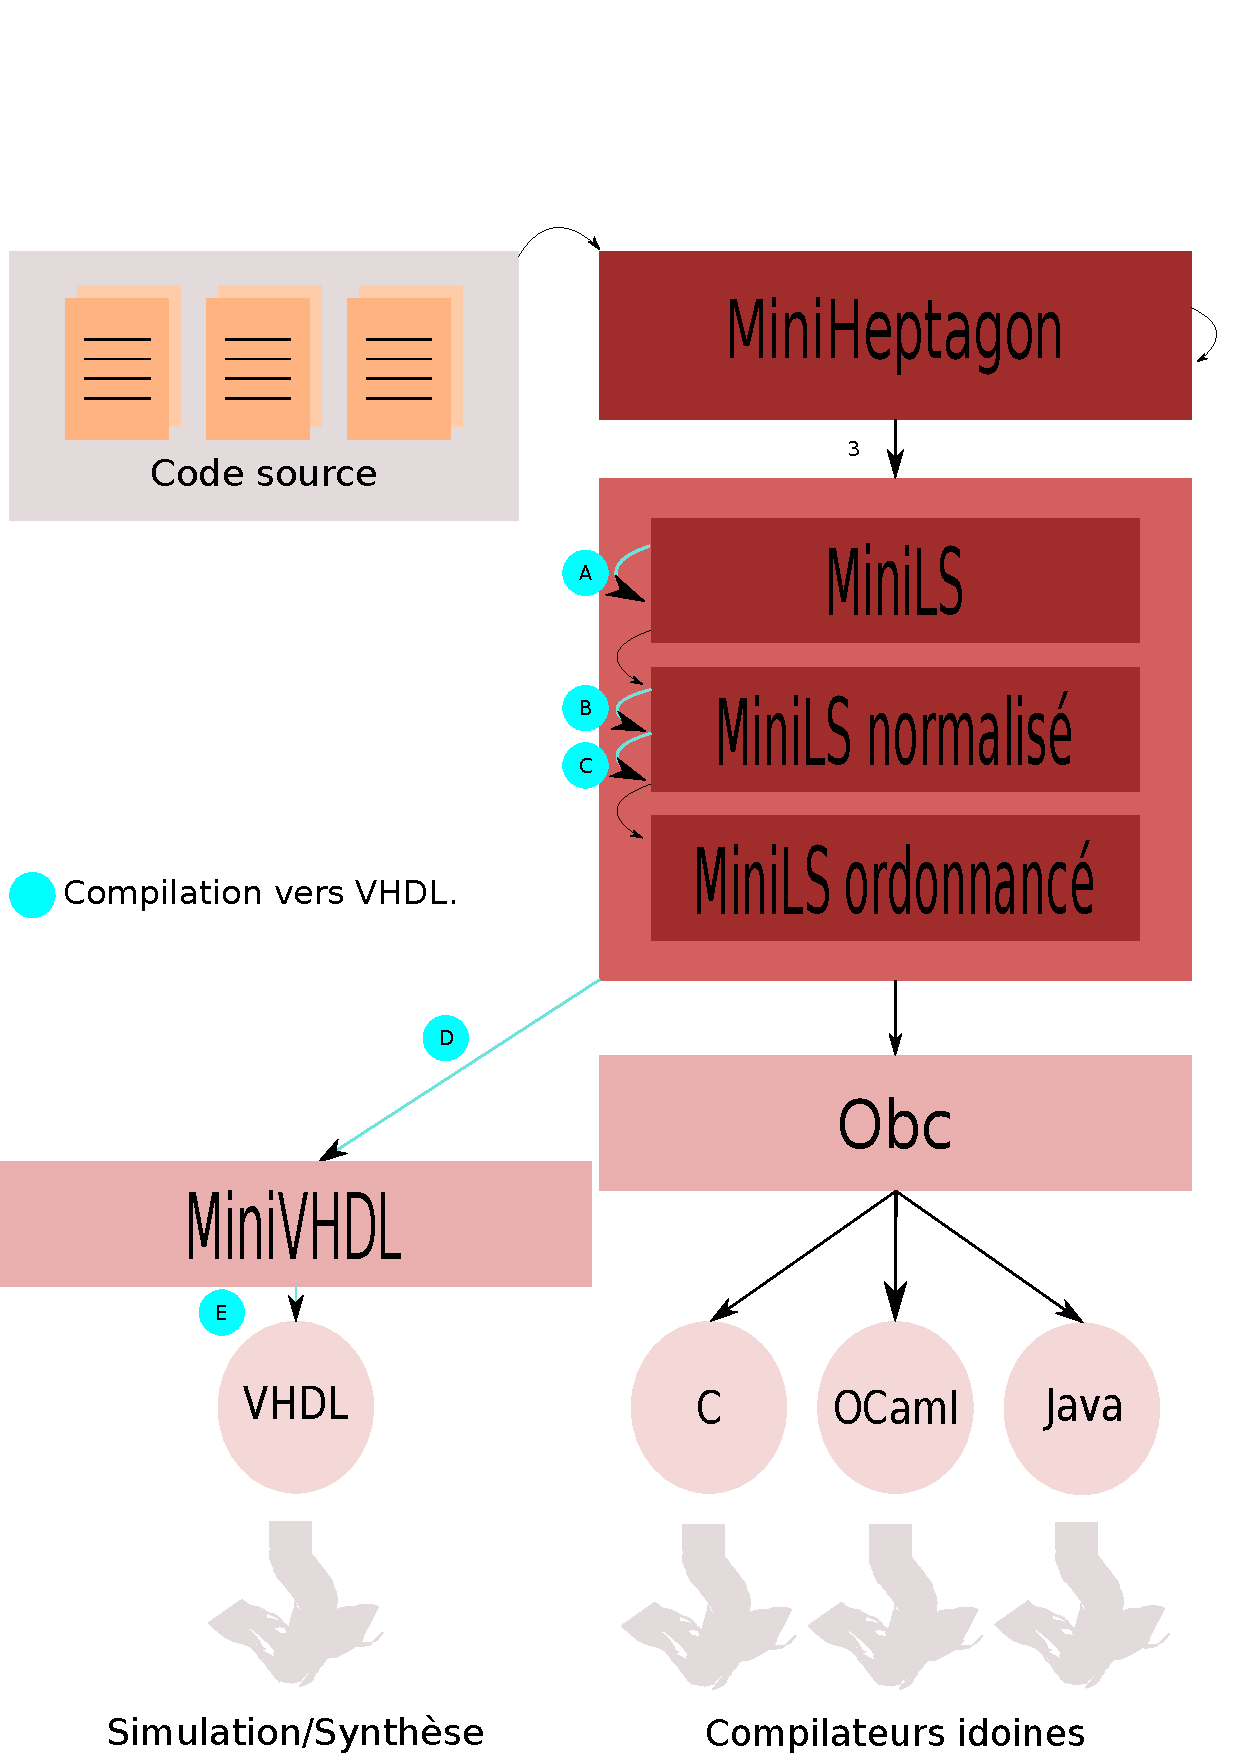
\includegraphics[scale=0.5]{archi}
  \caption{Architecture du compilateur \LANG}
  \label{fig:archi}
\end{figure}

Le passage au code séquentiel est court-circuité lors d'une compilation vers
\vhdl, qui traduit \minils{} directement vers celui-ci. Pour faciliter cette étape,
trois simplifications sont appliquées sur le code \minils.

\renewcommand{\labelenumi}{\Alph{enumi}}
\begin{enumerate}
\item suppression de la réinitialisation logique;
\item suppression des itérateurs par expansion de code;
\item introduction d'une variable intermédiaire pour chaque argument d'un appel
  de noeud.
\end{enumerate}
\renewcommand{\labelenumi}{\arabic{enumi}}

Le code obtenu sera finalement traduit vers un sous-ensemble de \vhdl, appelé
\minivhdl (à l'étape D), prêt à être traité par les outil dédiés (étape
E). Remarquons qu'il n'existe pas de définition précise identifiant un
sous-ensemble ``synthétisable'' du langage \vhdl, géré par les principaux outils
industriels. Après échange avec les partenaires du projet GENCOD, \minivhdl{}
correspond à un sous-ensemble raisonnable.


\section{De \LANG{} à VHDL}
Après avoir rappelé brièvement la forme des langages d'entrée et de sortie, on
va expliciter la procédure de traduction retenue.

\subsection{Langages internes}

\subsubsection{MiniLS}
\label{sec:syn:mls}

\begin{figure}[h]
  \centering
  \begin{eqnarray*}
    td & \Coloneqq & \mybox{type } bt = C + \dots + C \\
    d & \Coloneqq & \Node{p}{p}{p}{D} \\
    p & \Coloneqq & x : bt; \dots; x : bt \\
    D & \Coloneqq & pat = e; \dots; pat = e \\
    pat & \Coloneqq & x \p (pat,\dots,pat) \\
    e & \Coloneqq & x \p v \p \Op{e}{e} \p \Fby{v}{e} \p \Pre{e} \\
    & \p & \Every{f}{e}{e}{x} \p \When{e}{C}{x} \\
    & \p & \Merge{x}{C}{e}{C}{e} \\
    & \p & \Map{f}{e_1}{e_n} \\
    & \p & \Fold{f}{e_1}{e_n} \\
    & \p & \Mapfold{f}{e_1}{e_n} \\
    v & \Coloneqq & i \p C \\
    ck & \Coloneqq & \Base \p \On{ck}{C}{x}
  \end{eqnarray*}
  \caption{\minils}
  \label{fig:mls}
\end{figure}

\minils{} est un langage data-flow synchrone dans l'esprit de
\lustre~\cite{lustre:ieee91}, auquel on adjoint une construction de
réinitialisation modulaire et d'écrire des équations gardées par une
horloge. La compilation de \minils{} vers \vhdl{} passe successivement
par trois formes distinctes.

\begin{enumerate}
\item La forme originale (dont la syntaxe est définie dans la figure~\ref{fig:mls}) telle
  qu'obtenue à partir du code \LANG{} original.
\item Le code est traduit vers une forme normale
  (figure~\ref{fig:mlsn}).
\item La forme finale (voir figure~\ref{fig:mlsns}) est une forme
normalisée et dans laquelle les réinitialisations et les itérateurs de tableaux
ont été éliminés. De plus, les paramètres effectifs des appels de fonctions
sont nécessairement des noms de variables.
\end{enumerate}

\begin{figure}[htp]
  \centering
  \begin{eqnarray*}
    e & \Coloneqq & x \p v \p \Op{e}{e} \p \When{e}{C}{x} \\
    ce & \Coloneqq & e \p \Merge{x}{C}{ce}{C}{ce} \\
    eq & \Coloneqq & x = ce \p x = \Fby{v}{e} \p x = \Pre{e} \\
    & \p & (x,\dots,x) = \Every{f}{e}{e}{x} \\
    & \p & (x,\dots,x) = \App{f}{e,\dots,e} \\
    & \p & (x,\dots,x) = \Map{f}{e_1}{e_n} \\
    & \p & (x,\dots,x) = \Fold{f}{e_1}{e_n} \\
    & \p & (x,\dots,x) = \Mapfold{f}{e_1}{e_n}
  \end{eqnarray*}
  \caption{\minils normalisé}
  \label{fig:mlsn}
\end{figure}

\begin{figure}[htp]
  \centering
  \begin{eqnarray*}
    e & \Coloneqq & x \p v \p \Op{e}{e} \p \When{e}{C}{x} \\
    ce & \Coloneqq & e \p \Merge{x}{C}{ce}{C}{ce} \\
    eq & \Coloneqq & x = \Pre{e} \\
    & \p & (x,\dots,x) = \App{f}{x,\dots,x}
  \end{eqnarray*}
  \caption{\minils simplifié (et normalisé)}
  \label{fig:mlsns}
\end{figure}

\subsection{Sémantique intuitive}
La sémantique de \minils{} est celle de \lustre: un noeud est composé d'un ensemble
d'équations de suites mutuellement récursives. Discutons des points qui distinguent
le langage de \lustre:

\begin{itemize}
\item
Chaque expression $e$ est annotée par une expression d'horloge $ck$. $e$ doit
être calculée lorsque $ck$ est vrai. Cette annotation est produite automatiquement
par le compilateur au cours du calcul d'horloges.
\item
$\Every{f}{e_1}{e_n}{x}$ permet de réinitialiser l'appel de noeud $f^{ck}(e_1,...,e_n)$
lorsque $e$ est vraie.
\item
%% Les expressions simples du langage s'exécutent uniquement dans l'instant, et
%% n'ont pas d'effet en dehors de celui-ci.

%% \[
%% \begin{array}{|r|llllllllllllllllllllllllllll}
%%   \hline
%%   1     & 1 & 1 & 1 & 1 & \dots \\
%%   \hline
%%   1 + 2 & 3 & 3 & 3 & 3 & \dots \\
%%   \hline
%% \end{array}
%% \]

%% À l'inverse, les expressions \textrm{pre} et \textrm{fby} permettent de retarder
%% leur argument d'un instant, avec une valeur d'initialisation dans le cas de
%% \textrm{fby}.

%% \[
%% \begin{array}{|r|llllllllllllllllllllllllllll}
%%   \hline
%%   1 \ \mathrm{fby} \ 2 & 1 & 2 & 2 & 2 & \dots \\
%%   \hline
%%   \mathrm{pre} \ 3 &  & 3 & 3 & 3 & \dots \\
%%   \hline
%% \end{array}
%% \]

Les constructions \texttt{when} et \texttt{merge} permettent, appliquées à des expressions, de sous-échantillonner et sur-échantillonner ces dernières. L'emploi de ces
constructions a un effet sur les horloges: l'horloge de $\When{e}{C}{x}$ est
$\On{ck}{C}{x}$, où $ck$ est celle de $e$, et l'horloge de
$\Merge{x}{C_1}{e_1}{C_n}{e_n}$ est $ck$ quand celle des $e_i$ est
$\On{ck}{C}{x}$. L'expression $\On{ck}{C}{x}$ indique que le résultat est
présent lorsque l'horloge $ck$ est vraie et que $x$ est égal à $C$.

\[
\begin{array}{|r|llllllllllllllllllllllllllll}
  \hline
  x & 1 & 2 & 3 & 4 & \dots \\
  \hline
  h & false & true & false & true & \dots \\
  \hline
  \When{x}{true}{h} & & 2 & & 4 & \dots \\
  \hline
  u &  & 1 & & 4 & \dots \\
  \hline
  v & 0 & & 3 & & \dots \\
  \hline
  \Merges{h}{true}{u}{false}{v} & 0 & 1 & 3 & 4 \\
  \hline
\end{array}
\]

\item
Les itérateurs \texttt{map}, \texttt{fold}, et \texttt{mapfold}
prennent en argument une fonction $f$, une taille de tableau et un ou
plusieurs tableaux. La sémantique de ces constructions est celle
donnée dans~\cite{lucy:genie00,morel-07-jes}.

\begin{itemize}
\item \texttt{map} applique en parallèle $f$ à tous les éléments des tableaux
  pour former un nouveau tableau.
\item \texttt{fold} applique en série $f$ sur tous les éléments d'un tableau en
  passant un accumulateur et renvoie ce dernier une fois le parcours terminé.
\item \texttt{mapfold}, qui suppose que $f$ renvoie au moins deux valeurs,
  combine les deux en construisant un nouveau tableau avec le premier résultat
  de $f$ (à la manière de \texttt{map}) et en passant un accumulateur durant le
  parcours (tout comme \texttt{fold}).
\end{itemize}
\end{itemize}

\subsubsection{MiniVHDL}

\minivhdl{} (défini dans la figure~\ref{fig:mvhdl})
est un fragment de \vhdl{} suffisant pour
décrire l'essence du processus de traduction. Un composant \minivhdl:
\[
\Component{f}{P}{sigs}{lvars}{ports}{I}
\]
correspond à un
composant \vhdl{} formé des instantiations $ports$, signaux internes $sigs$ et d'un
processus avec les variables locales $lvars$ et de corps $I$.

Le langage est structuré sous forme de composants. Chacun d'eux possède des
signaux d'entrée et de sortie, des signaux locaux, des variables locales, d'éventuels
sous-composants, et enfin un corps formé d'une suite d'instructions.

La sémantique informelle du langage est la suivante: dès que la valeur d'un
signal d'entrée ou local change, le corps du composant est exécuté. Celui-ci
peut modifier la valeur d'autres signaux via l'instruction $x \Leftarrow e$ ($x$
étant par définition un signal), entraînant ainsi l'activation de
sous-composants, ou même la réactivation du composant courant. Les variables
locales sont semblables aux variables des langages de programmation
traditionnels: elles n'ont de valeur que pendant l'exécution du corps d'un
composant. L'exécution s'arrête une fois tous les signaux stables.

\begin{figure}[t]
  \centering
  \begin{eqnarray*}
    component & \Coloneqq & \mybox{component} \; f \; \mybox{port} \; sm;\dots;\
    sm \; \mybox{with} \, \mybox{sig} \; d; \dots; d \; \\
    & & \mybox{and} \, \mybox{var} \; d; \dots; d \; \mybox{and} \
    \mybox{subcomponents} \; p; \dots; p \; \mybox{in} \; I \\
    sm & \Coloneqq & x : mode \ ty \\
    sd & \Coloneqq & x : mode \ ty := e \\
    mode & \Coloneqq & \mybox{in} \p \mybox{out} \\
    d & \Coloneqq & x : ty \\
    p & \Coloneqq & \mybox{port map } x (bd;\dots;bd) \\
    bd & \Coloneqq & x \Rightarrow x \\
    I & \coloneqq & i; \dots; i \\
    i & \Coloneqq & \Assign{x}{e} \p \Affect{x}{e} \p \Case{e}{v}{I}{v}{I} \\
    e & \Coloneqq & id \; \vert \; v \; \vert \; \Op{e}{e} \\
    v & \Coloneqq & i \; \vert \; ' bitp ' \\
    bitp & \Coloneqq & bit \p bit \  bitp \\
    bit & \Coloneqq & \mathbf{0} \p \mathbf{1} \\
    bt & \Coloneqq & \mybox{natural} \p \mybox{std\_logic} \p \mybox{bit}
    \p \dots
  \end{eqnarray*}
  \caption{MiniVHDL}
  \label{fig:mvhdl}
\end{figure}

Notons que les paramètres effectifs des sous-composants sont des noms de
signaux; cela justifie la forme simplifiée \minils{} décrite précédemment.

\subsection{Simplification de MiniLS normalisé}

Nous effectuons donc trois passes pour simplifier le code \minils.

\subsubsection{Élimination de la réinitialisation logique}

Comme expliqué plus haut, certaines constructions de \minils{} proposent au
programmeur une forme de réinitialisation modulaire : les équations de la
forme $\Fby{v}{e}$ d'un noeud $f$ instancié par la construction
$\Every{f}{e_1}{e_n}{z}$ doivent être réinitialisées dès lors que $z$
est vrai.

La première passe de simplification, qui s'exécute sur le code \minils{}
obtenu à la troisième étape du processus décrit plus haut, va exprimer
la réinitialisation en fonction du reste du langage, réduisant ainsi la
complexité du langage à traduire vers \vhdl{}.

On va supposer dans ce qui suit que l'identificateur \textbf{rst} est un
identificateur utilisé nulle part dans le programme. En pratique, le compilateur
s'assure de l'absence de conflit avec les variables de l'utilisateur.

L'idée est d'ajouter à chaque noeud un argument supplémentaire nommé
\textbf{rst} qui vaudra $true$ lorsqu'une réinitialisation de la mémoire est
nécessaire, et de modifier les expressions contenant des constructions
\texttt{fby} ou \texttt{every} pour prendre en compte \textbf{rst}. L'exemple
suivant reprend le compteur simple présenté plus haut pour illustrer cette
simplification.

\verbatiminput{rst_ex.ept}

Une fois le reset éliminé, le code est le suivant :

\verbatiminput{rst_ex2.ept}

On va détailler les fonctions effectuant ces deux tâches : $RstE(e)$ prend
une expression \minils{} $e$ et renvoie une nouvelle expression où la
réinitialisation a été éliminée, et $RstNode(nd)$ prend un nœud $nd$
et renvoie un nouveau nœud prenant un \texttt{rst} à un noeud et transforme
ses équations.

\newcommand{\re}[1]{RstE(#1)}
\newcommand{\rstn}[1]{RstNode(#1)}

\[
\begin{array}{lcl}
  \re{\Op{e_1}{e_n}} & = & \Op{\re{e_1}}{\re{e_n}} \\
  \re{\Fby{v}{e}} & = & \If{rst}{v}{(\Fby{v}{\re{e}})} \\
  \re{\Pre{e}} & = & \Pre{\re{e}} \\
  \re{\Every{f}{e_1}{e_n}{x}} & = & \App{f}{\mathbf{rst} \; \mathtt{or} \;
    x, \re{e_1} \dots, \re{e_n}} \\
  \re{\App{f}{e_1,\dots,e_n}} & = &
  \App{f}{\mathbf{rst},\re{e_1},\dots,\re{e_n}} \\
  \re{\If{e_1}{e_2}{e_3}} & = & \If{\re{e_1}}{\re{e_2}\\ & & \hspace{1.9cm}}
  {\re{e_3}} \\
  \re{\When{e}{C}{x}} & = & \When{\re{e}}{C}{x} \\
  \re{\Merge{e}{C_1}{e_1}{C_n}{e_n}} & = &
  \mybox{merge} \; \re{e} \; (C_1 \Rightarrow \re{e_1}) \\
  & & \hspace{2.4cm} \dots \\
  & & \hspace{2.4cm} (C_n \Rightarrow \re{e_n})
\\ \\
RstEqs(pat_1 = e_1;\dots;pat_n = e_n) & = &
  pat_1 = \re{e_1};\dots;pat_n = \re{e_n} \\
  \end{array}
\]

\[
\begin{array}{ll}
  \rstn{\Node{f}{x_1,\dots,x_n}{y_1,\dots,y_n}{eqs}} & = \\
  \ind \Node{f}{rst,x_1,\dots,x_n}{y_1,\dots,y_n}{ResetEqs(eqs)}
\end{array}
\]

\subsubsection{Suppression des itérateurs}

La version actuelle du compilateur et de son générateur de code \vhdl{} supporte
les tableaux de dimension arbitraire \footnote{En pratique, les outils de
  synthèse de circuits à partir de code \vhdl{} imposent une dimension maximale.}
et constructions associées ; il nous faut donc compiler les itérateurs
\texttt{map}, \texttt{fold} et \texttt{mapfold} vers \vhdl{}.

Par souci de simplicité et uniformité, nous avons fait le choix de les
éliminer par expansion lors d'une transformation source-à-source sur
\minils. On ne détaillera pas cette opération qui consiste simplement à
remplacer les itérateurs par plusieurs équations. L'équation $x =
\Map{f}{t_1}{t_m}$ lorsque les tableaux $t_1, \dots, t_m$ sont de taille $n$
sera ainsi remplacée par $n + 1$ équations dont les $n$ premières
effectuent l'application de $f$ pour chaque indice et la dernière affecte à
$x$ le tableau en résultant. On applique des transformations similaires aux
opérateurs \texttt{fold} et \texttt{mapfold}.

Le programme suivant présente un exemple effectuant un ET logique sur tous les
éléments d'un tableau via l'itérateur \texttt{fold}.

\verbatiminput{fold_orig.ept}

Son pendant avec itérateur mis à plat se contente de passer l'accumulateur
d'élément en élément.

\verbatiminput{fold_il.ept}

Un traitement spécial est adopté pour l'utilisation de \texttt{map} avec
certains opérateurs. En effet, \vhdl{} permet d'utiliser certains opérateurs sur
des tableaux de bits, sans avoir à déconstruire ces derniers ; par exemple, il
est possible d'effectuer un ET logique bit-à-bit sur deux tableaux $t_1$ et
$t_2$ via $t_1 \ \texttt{and} \ t_2$. La passe effectue la transformation de
$\texttt{map}\ \textbf{op}<<n>>(t_1,\dots,t_n)$ à $t_1\ \textbf{op}\ \dots
\textbf{op}\ t_n$ lorsque cela est possible.

\subsubsection{Simplification des appels}

\newcommand{\simpl}[2]{Simpl(#1,#2)}
\newcommand{\simplnd}[1]{SimplNode(#1)}

Comme nous le verrons plus bas, les appels de nœuds seront compilés en
instantiations de composants ; or, les arguments d'une construction \vhdl{}
$port \; map$ sont forcément des identificateurs. Pour simplifier la
génération de \vhdl{}, on va donc modifier en amont chaque appel de noeud en
introduisant une variable intermédiaire pour chaque argument. La fonction
$\simpl{eq}{eqs}$ simplifie l'équation $eq$ en ajoutant la ou les équations
produits à la liste des équations déjà traitées $eqs$ ; $\simplnd{nd}$
prend un noeud $nd$ et simplifie les appels présents dans ses équations. Le
symbole $\Cons$ dénote la concaténation en tête de liste.

\[
\begin{array}{ll}
  \simpl{x = ce}{eqs} & = \\
  \ind (x = ce) \Cons eqs \\
  \simpl{x = \Pre{e}}{eqs} & = \\
  \ind (x = \Pre{e}) \Cons eqs \\

  \simpl{(x_1,\dots,x_n) = \App{f}{e_1,\dots,e_n}}{eqs} & = \\
  \ind (y_1 = e_1) \Cons \dots \Cons (y_n = e_n)
  \Cons ((x_1,\dots,x_n) = \App{f}{rst,y_1,\dots,y_n}) \Cons eqs \\
  \ind \mbox{où } y_1,\dots,y_n \mbox{ sont des noms de variables frais}
\end{array}
\]

\[
\begin{array}{ll}
  \simplnd{\Node{x_1,\dots,x_n}{y_1,\dots,y_n}{p}{D}} & = \\
  \ind \mathtt{node} f(x_1,\dots,x_n) = y_1, \dots, y_n \; \\
  \ind \mathtt{with} \  \mathtt{var} \; p' \; \mathtt{in} \; fold\_right \;Simpl
  \; D \; [] \\
  \ind \mbox{en supposant que $p'$ correspond
             aux variables définies par} \\ \ind \mbox{les nouvelles équations.}
\end{array}
\]

Ces simplifications effectuées, le programme résultant est traduit vers \minivhdl.

\subsection{MiniLS simplifié vers MiniVHDL}

Le principe général de la traduction de \minils{} simplifié vers \minivhdl{} est le
suivant:

\begin{enumerate}
\item Chaque noeud \minils{} correspondra à un composant \minivhdl.
\item Chaque équation à mémoire (i.e. contenant $fby$ ou $pre$) va correspondre
  à un signal \vhdl{} local, chaque équation combinatoire à une variable locale.
\item Les horloges importent uniquement pour les équations de la forme $x =
  \Fby{v}{e}$ et $(x_1,\dots,x_n) = \App{f}{e_1,\dots,e_n}$ : il faudra alors
  générer la garde booléenne correspondant à $ck$. Les autres sont combinatoires
  et ne nécessitent pas de traitement particulier.
\item La réinitialisation logique est gérée en amont comme expliquée ci-dessus,
  elle est donc implicitement asynchrone (indépendante des fronts montants de
  l'horloge).
\item Les partenaires ont exprimé le désir de pouvoir réinitialiser
  physiquement toute la mémoire lors du basculement d'un signal précis
  nommé \textbf{hwrst} : on ajoute donc ce signal supplémentaire
  invisible dans le code \minils{} et on génère le code de
  réinitialisation correspondant lors du traitement du $fby$. Tout
  comme pour l'identificateur \textbf{rst} plus haut, on suppose que
  l'identificateur \textbf{hwrst} n'est pas utilisé dans le programme.
\item Pour respecter la sémantique à $\Delta$-cycles de \vhdl{}, il importe de
  faire évoluer la mémoire par un pas du calcul uniquement sur front montant de
  l'horloge.
\item En suivant le modèle synchrone, les valeurs calculées par le circuit à
  d'autres moments que le front montant n'ont pas de sens bien défini ; on les
  ignorera donc.
\item Chaque appel de noeud correspondra à une instantiation. Comme spécifié
  plus haut, les paramètres effectifs d'un signal \vhdl{} sont obligatoirement des
  signaux auxquels il faudra assigner la valeur correcte.
\end{enumerate}

\subsubsection{Traduction des types}

Les déclarations de types de données ont été laissées implicites aussi bien dans
la syntaxe de \minils{} que de \minivhdl{} ; les possibilités étant exactement les
mêmes (énumérations et enregistrements), on choisit de ne pas s'attarder sur
leur traduction qui reste une traduction mot-à-mot d'une syntaxe concrète à
l'autre.

\subsubsection{Traduction des constantes et fonction auxiliaires sur les horloges}

La fonction $TradConst(c)$ traduit une constante \minils{} $c$ en constante
\minivhdl{}.

\newcommand{\TradC}[1]{TradConst(#1)}

\[
\begin{array}{lcl}
  \TradC{i} & = & i \\
  \TradC{true} & = & '1' \\
  \TradC{false} & = & '0' \\
  \TradC{C} & = & C
\end{array}
\]

La fonction auxiliaire $GuardClock$ permet de traduire une horloge \minils{} en
expression \minivhdl{} de type booléen. Elle sera utilisée pour contrôler la
mise à jour des registres, s'assurant que cette dernière n'est effectuée
qu'aux instants où l'horloge est effective.

\newcommand{\GEC}[1]{GuardClock(#1)}

\[
\begin{array}{lcl}
  \GEC{\Base} & = & rising\_edge(clk) \\
  \GEC{\On{ck}{C}{x}} & = & x = \TradC{C} \; \mathtt{and} \; \GEC{ck}
\end{array}
\]

Tout comme les mises à jour des mémoires, les appels à d'autres noeuds
sont dirigés par les horloges qui en donnent la cadence. Il nous faudra donc
une fonction voisine de $GuardClock$ pour calculer l'expression \minivhdl{}
correspondant à l'horloge utilisée dans l'appel d'un noeud.

\newcommand{\EC}[1]{ExpClock(#1)}

\[
\begin{array}{lcl}
  \EC{\Base} & = & clk \\
  \EC{\On{ck}{C}{x}} & = & x = \TradC{C} \; \mathtt{and} \; \EC{ck}
\end{array}
\]

\subsubsection{Traduction des expressions et équations}

La fonction $TradExp(e)$ traduit l'expression \minils{} normalisée et
simplifié $e$ en expression \minivhdl{}.

\newcommand{\TradE}[1]{TradExp(#1)}

\[
\begin{array}{lcl}
  \TradE{v} & = & \TradC{v} \\
  \TradE{x} & = & x \\
  \TradE{\Op{e_1}{e_n}} & = & \Op{\TradE{e_1}}{\TradE{e_n}} \\
  \TradE{\When{e}{C}{x}} & = & \TradE{e}
\end{array}
\]

La construction \texttt{when} n'a pas de sens calculatoire, et peut n'être vue
que comme une annotation d'horloge. Elle sera ignorée lors du processus de
traduction.

La fonction $TradCExp(ce)$ traduit les expressions $ce$ de contrôle formées
d'expressions simples ou de \texttt{merge} imbriqués en instructions \minivhdl{}.

\newcommand{\TradCE}[2]{TradCExp(#1, #2)}

\[
\begin{array}{ll}
  \TradCE{x}{\Merge{y}{C_1}{ce_1}{C_n}{ce_n}} & = \\
  \ind \mathtt{case} \; y \; \mathtt{of} \;
  (\TradC{C_1} \Rightarrow \TradCE{x}{ce_1}) \\
  \hspace{2.1cm} \dots \\
  \hspace{2.1cm} (\TradC{C_n} \Rightarrow \TradCE{x}{ce_n}) \\
  \TradCE{x}{e} & = \\
  \ind \Affect{x}{\TradE{e}}
\end{array}
\]

Enfin, la fonction $TradEq$ permet de passer des équations aux instructions
\minivhdl{}. Elle prend un argument supplémentaire permettant de compter le nombre
d'appels de noeuds afin de générer des arguments supplémentaires, et on se donne
une fonction supplémentaire $MakeArg(x,i)$ qui génère un nom de variable frais à
partir du nom de variable $x$ et de l'entier $i$.

La traduction des équations appelant un noeud nécessite des explications
concernant la fa\c{c}on de compiler les appels d'un noeud \minils{} qui seront données
à la section suivante.

\newcommand{\TradEq}[2]{TradEq(#1,#2)}
\newcommand{\MA}[2]{MakeArg(#1,#2)}

\[
\begin{array}{lcl}
  \TradEq{x = ce}{i} & = & \TradCE{x}{ce}, i \\

  \TradEq{x = \Pre{e}}{i} & = & \mathtt{if} \; \GEC{ck} \; \mathtt{then} \\
  & & \ind \Assign{x}{\TradE{e}} \\
  & & \mathtt{end} \; \mathtt{if}, i \\

  \TradEq{x = \Fby{y}{e}}{i} & = & \mathtt{if} \; \mathbf{hwrst}
  \; \mathtt{then} \\
  & & \ind \Assign{x}{y} \\
  & & \mathtt{elsif} \; \GEC{ck} \; \mathtt{then} \\
  & & \ind \Assign{x}{\TradE{e}} \\
  & & \mathtt{end} \; \mathtt{if}, i \\


  \TradEq{(x_1,\dots,x_n) = \App{f}{y_1,\dots,y_n}}{n} & = &
  \Assign{\MA{"ck"}{i}}{\EC{ck}} \\
  & & \Assign{\MA{y_1}{i}}{y_1} \\
  & & \dots \\
  & & \Assign{\MA{y_n}{i}}{y_n}, i + 1 \\
\end{array}
\]

Précisons que par construction, l'interface d'un composant suit toujours la
forme suivante:
\[(clk, hwrst, in_1, \dots,in_n, out_1,\dots,out_n)
\]
Rappelons que le reset ``logique'' (celui utilisé dans les automates, par exemple
ou la construction \verb-every-) est maintenant une entrée supplémentaire (ici $in_1$).

\subsubsection{Gestion des tableaux}

Hormis le cas des itérateurs traités précédemment, la gestion des
tableaux n'appelle pas de commentaire particulier, à l'exception de la
nécessité de déclarer à l'avance les types tableaux (bornes exclues) en
\vhdl{}. Deux solutions sont envisageables:

\begin{itemize}
\item Calculer la dimension maximale des tableaux rencontrés dans le programme,
  et utiliser cette information pour pré-déclarer les tableaux \vhdl{} idoines.
\item Déclarer quoi qu'il advienne les types de tableaux utiles et refuser les
  programmes comprenant des dimensions supérieures à une limite fixée à l'avance.
\end{itemize}

Le compilateur emploie pour l'instant la première méthode mais la seconde ne
nous semble pas dérangeante pour des raisons pragmatiques~\footnote{Notons que
  notre version de l'outil Xilinx ISE refuse tout tableau de
  dimension supérieure à trois.}.

\subsubsection{Compilation modulaire et appels de noeuds}

\minivhdl{} offre une forme de modularité basée sur une hiérarchie de
composants. Chacun de ces derniers spécifie une liste de composants fils dont
les ports (au sens de la figure \ref{fig:mvhdl}) sont instantiés avec des
signaux. Nous prenons donc soin d'utiliser des signaux comme résultats mais
aussi arguments ; par souci de simplicité, on introduit des signaux locaux
pour chaque argument, signaux qui seront affectés lors de la traduction de
l'équation correspondant à l'appel de noeud original.

La fonction $GatherPortMaps(D, i)$ rassemble cette liste de sous-noeuds à
partir des appels de noeud présents dans le paquet d'équations $D$ et
créé les instantiations de composants correspondantes. L'entier $i$ nous
servira à distinguer les appels de noeuds et de créer de nouveaux noms de
signaux frais grâce à la fonction $MakeArg$ décrite plus haut. On se donne
également une fonction $GetArgName(f,n)$ qui renvoie le nom du $n$-ème
argument du noeud de nom $f$.

\newcommand{\GPM}[2]{GatherPortMaps(#1,#2)}
\newcommand{\GAN}[2]{GetArgName(#1,#2)}

\[
\begin{array}{lcl}
  \GPM{[]}{i} & = & [] \\
  \GPM{((x_1,\dots,x_n) = \App{f}{y_1,\dots,y_n}) \Cons eqs}{i} & = &
  \\
  \ind \mybox{port map} \; f ( clk \Rightarrow \MA{"clk"}{i} \\
  \ind \ind \ind \ind \hspace{0.4cm} \GAN{f}{1} \Rightarrow \MA{y_1}{i} \\
  \ind \ind \ind \ind \hspace{0.4cm} \dots \\
  \ind \ind \ind \ind \hspace{0.4cm} \GAN{f}{n} \Rightarrow \MA{y_n}{i}) \\
  \ind \Cons \GPM{eqs}{i + 1}
\end{array}
\]

On définit ensuite les fonctions auxiliaires $NeedVar$, $Vars$, $ParamSigs$ et
$SignalOfVarDec$ respectivement chargées de déterminer si une équation introduit
des déclarations de variables locales ou non, de calculer la liste des variables
définies par une équation, de calculer les signaux à passer en arguments aux
appels de noeuds présents dans un paquet d'équations et enfin de traduire
simplement une déclaration de variable \minils{} en déclaration de signal \minivhdl{}
avec mode d'utilisation (entrée ou sortie).

\newcommand{\NV}[1]{NeedVar(#1)}
\newcommand{\V}[1]{Vars(#1)}
\newcommand{\PS}[2]{ParamSigs(#1,#2)}
\newcommand{\SoVD}[3]{SignalOfVarDec(#1 : #2, #3)}

\[
\begin{array}{lcl}
  \NV{x = \Fby{v}{e}} & = & false \\
  \NV{(x_1,\dots,x_n) = \App{f}{y_1,\dots,y_n}} & = & false \\
  \NV{x = ce} & = & true
\end{array}
\]

\[
\begin{array}{lcl}
  \V{x = \Fby{v}{e}} & = & [x] \\
  \V{(x_1,\dots,x_n) = \App{f}{y_1,\dots,y_n}} & = & x_1 \Cons \dots \Cons x_n \\
  \V{x = ce} & = & [x]
\end{array}
\]

\[
\begin{array}{ll}
  \PS{x = \Fby{v}{e} \Cons eqs}{i} & = \\
  \ind \PS{eqs}{i} \\
  \PS{(x_1,\dots,x_n) = \App{f}{y_1,\dots,y_n} \Cons eqs}{i} & = \\
  \ind \MA{"clk"}{i} \Cons \MA{y_1}{i} \Cons \dots \Cons \MA{y_n}{i} \\
  \ind \mathtt{::} \; \PS{eqs}{i + 1}
  \\
  \PS{x = ce \Cons eqs}{i} & = \\
  \ind \PS{eqs}{i}
\end{array}
\]

\[
\begin{array}[lcl]{lcl}
  \SoVD{x}{bt}{mode} & = & \mybox{signal} \; x : mode \; TransBaseType(bt)
\end{array}
\]

\subsubsection{Traduction des noeuds}

Enfin, $TradNode(nd)$ se charge de traduire un noeud $nd$ en composant
\minivhdl{}, en créant un signal local pour chaque équation retardée et
argument d'appel de noeud, une variable pour chaque équation combinatoire, et
la liste de sous-composants requise.

\begin{align*}
  & TradNode(\mybox{node } f(in) = out \mybox{ with var } p \mybox{ in } D) = \\
  & \bl \mbox{soit } port = \\
  & \bl \bl clk : \mybox{in std\_logic}; \\
  & \bl \bl \{ SignalOfVarDec(x : bt, \mybox{in}) \p (x : bt) \in in \}; \\
  & \bl \bl \{ SignalOfVarDec(x : bt, \mybox{out}) \p (x : bt) \in out \}, \\
  & \bl \mbox{ soit } signals = \{ \V{eq} \p eq \in D, \neg \NV{eq} \}
  \mybox{,} \\
  & \bl \mbox{ soit } sig\_args = \PS{D}{1} \mybox{,} \\
  & \bl \mbox{ soit } variables = \{ \V{eq} \p eq \in D, \NV{eq} \} \mybox{,} \\
  & \bl \mbox{ soit } ports = \GPM{D}{1} \mybox{,} \\
  & \bl \mbox{ soit } body = fold\_right TradEq D ([], 1) \mbox{ dans} \\
  & \mybox{component } f \mybox{ port } port \mybox{ with sig } signals \cup
  sig\_args \\
  & \mybox{and var } variables \mybox{ and subcomponents } ports \mybox{ in }
  body
\end{align*}

\section{Conclusion}

Ce document décrit les étapes de traduction d'un langage proche de
\scade{} vers un sous-ensemble de \vhdl. Le processus s'applique
directement sur un format intermédiaire data-flow. Le code chargé de la traduction
de \minils{} vers \minivhdl{} est court (de l'ordre de 600 lignes de code OCaml).
Notons que le compilateur réalisé est capable d'assurer le retour au source (tra\c{c}abilité)
depuis le code \LANG{} (conservation des identificateurs et de leur renommage
au cours des étapes de compilation).

Plusieurs exemples fournis par les membres du projet ont été expérimentés. L'efficacité
du code obtenu semble comparable au code produit par Geensoft. Une expérience plus
poussée pourrait être menée à l'avenir. 

\newpage
\tableofcontents

\newpage
\bibliographystyle{plain}
\bibliography{lucy,synchrone,biblio}

\newpage
\appendix


\section{Exemples de code généré}

On présente ici quelques codes générés par notre prototype. En l'état
actuel de ce dernier, beaucoup de variables intermédiaires inutiles sont
générées ; cela s'explique pour deux raisons :

\begin{itemize}
\item Ces codes représentent des sorties brutes n'ayant subies aucune
  optimisation.
\item Certaines passes du compilateur ont naturellement tendance à introduire
  des variables intermédiaire de fa\c{c}on préventive, simplifiant ainsi leur
  fonctionnement.
\end{itemize}

\subsection{Compteur}

\paragraph{MiniLS initial}

\small
\verbatiminput{compteur2_init.mls}
\normalsize

\paragraph{MiniLS normalisé, ordonnancé et simplifié}

Notons que le noeud \textit{compteur} est ici instancié avec son paramètre
\textit{n} égal à 4, ceci afin de pouvoir déplier les itérateurs.

\small
\verbatiminput{compteur2_sched.mls}
\normalsize

\paragraph{VHDL}

\small
\verbatiminput{compteur2_vhdl.vhd}
\normalsize

\subsection{Allocateur de ressource}

\paragraph{MiniLS initial}

\small
\verbatiminput{al2_init.mls}
\normalsize

\paragraph{MiniLS normalisé, ordonnancé et simplifié}

\small
\verbatiminput{al2_sched.mls}
\normalsize

\paragraph{VHDL}

\small
\verbatiminput{al2_vhdl.vhd}
\normalsize

\section{Utilisation du compilateur}

Nous supposerons dans ce manuel que l'archive du compilateur a été
décompressée dans le répertoire \verb/$HEPTDIR/. Cette archive contient le
présent rapport, un répertoire \texttt{exs/} avec une batterie d'exemples
\LANG{} compilés vers \vhdl{}, et un binaire en code-octet pour la machine
abstraite OCaml. Ce dernier peut-être exécuté via \texttt{ocamlrun heptc},
ou bien directement lorsque votre \texttt{ocamlrun} est présent dans
\texttt{/usr/bin}. Nous supposerons par la suite que c'est le cas et que votre
variable d'environnement \verb/$PATH/ contient \verb/$HEPTDIR//bin.

Pour utiliser le compilateur, il faut tout d'abord renseigner la variable
d'environnement \verb/$HEPTLIB/ spécifiant au compilateur où trouver la
bibliothèque standard.

\begin{verbatim}
$ export HEPTLIB=$HEPTDIR/lib
\end{verbatim}

Vous pouvez ensuite vérifier que le compilateur est disponible et fonctionnel
via la commande suivante :

\begin{verbatim}
$ heptc -version
The Heptagon compiler, version 0.4 (wed. aug. 18 11:17:42 CET 2010)
Standard library in [...]
\end{verbatim}

Pour compiler un fichier \LANG, le compilateur doit être invoqué avec l'option
\verb/-target/. Les arguments possibles pour cette option sont :

\begin{itemize}
\item \verb/vhdl/ : génère du code \vhdl{}.
\item \verb/mls/ : génère le code à flots de données \minils{} intermédiaire.
\item \verb/obc/ : génère un code impératif simple dans le langage idéalisé Obc.
\item \verb/c/ : génère du code C.
\end{itemize}

Les cibles \vhdl{} et C invoquées sur un fichier \verb/source.ept/ produisent
respectivement un dossier \verb/source_vhdl/ et \verb/source_c/ qui contiennent
les fichiers sources générés. Par exemple :

\begin{verbatim}
$ cat source.ept
node main() returns (o : int)
let
  o = 0 fby (o + 1);
tel
$ heptc -target vhdl source.ept
$ ls source_vhdl
main.vhd  types.vhd
\end{verbatim}

L'option \verb/-s noeud/ permet de générer le code nécessaire à un
exécutable autonome à partir d'un fichier source \LANG, c'est à dire un
\textit{test-bench} dans le cas de \vhdl{} et une fonction \verb/main()/ en ce
qui concerne C. Voici un exemple d'utilisation de la sortie C :

\begin{verbatim}
$ cat source.ept
node noeud() returns (o : int)
let
  o = 0 fby (o + 1);
tel

node main() returns (o : int)
let
  o = noeud() + 1;
tel
$ heptc -target c -s main source.ept
$ ls source_c
_main.c  _main.h  source.c  source.h  source_types.c  source_types.h
$ cc -Isource_c source_c/*.c -o source
$ ./source 5 # Option indiquant a l'executable genere de s'arreter apres 5 pas
=> 1
=> 2
=> 3
=> 4
=> 5
\end{verbatim}

\section{Grammaire de Heptagon}

Cette grammaire de référence explicite la syntaxe du langage \heptagon.

\newcommand{\sdash}{\mbox{-}}
\newcommand{\spow}{\text{\^{ }}}
\newcommand{\piquots}[1]{<<#1>>}

\newcommand{\lp}{\texttt{(}}
\newcommand{\rp}{\texttt{)}}
\newcommand{\lcb}{\texttt{\{}}
\newcommand{\rcb}{\texttt{\}}}

\[
\begin{array}{lcl}
  type & \Coloneqq & \mathtt{int} \p \mathtt{bool} \p \mathtt{float} \p
    {\bf type\sdash{}name} \\
  & | & type \spow{} constant \\

  \\

  constant & \Coloneqq & {\bf constant\sdash{}name} \\
  & | & {\bf integer} \\
  & | & {\bf string} \\
  & | & constant + constant \\
  & | & constant - constant \\
  & | & \dots \\

  \\

  expression & \Coloneqq & constant \\
  & | & {\bf variable\sdash{}name} \\
  & | & expression + expression \p expression - expression \p \dots \\
  & | &
    iterator \  \lp{}iterator\sdash{}argument\rp{}
    \piquots{constant} \lp{}expression^+\rp{}
    \\
  & | &
    {\bf function\sdash{}name} \; static\sdash{}parameters \;
    \lp{}expression,\dots,expression\rp{} \\
  & | & \mathtt{last} \  {\bf variable\sdash{}name} \\
  & | & \mathtt{pre} \  expression \\
  & | & constant \  \mathtt{fby} \  expression \\
  & | & expression \  \texttt{->} \  expression \\
  & | & \lp{}expression,\dots,\ expression\rp{} \\
  & | & expression = expression \\
  & | & \mathtt{if} \ expression \ \mathtt{then} \ expression \ 
    \mathtt{else} \ expression \\
  & | & \lcb{} field\sdash{}def^+ \rcb{} \\
  & | & expression.{\bf field\sdash{}name} \\
  & | & \lcb{} expression
    \ \mathtt{with} \  field\sdash{}def^+ \rcb{} \\
  & | & [ expression, \dots, expression ] \\
  & | & expression \spow{} constant \\
  & | & expression.[constant^+] \\
  & | & expression.[constant \  .. \ constant] \\
  & | & expression.[expression^+] \ \mathtt{default} \  expression \\
  & | & [ expression \ \mathtt{with} \ expression^+ \ = \ expression ] \\
  & | & expression \ @ \ expression \\

  \\

  static\sdash{}parameters & \Coloneqq & \epsilon \\
  & | & \piquots{constant,\dots,constant} \\

  \\

  iterator & \Coloneqq & \mathtt{map} \p \mathtt{fold} \p \mathtt{mapfold} \\
  iterator\sdash{}argument & \Coloneqq &
    {\bf function\sdash{}name} \; static\sdash{}parameters
    \p \mathtt{+} \p \mathtt{-} \p \dots \\

  \\

  field\sdash{}def & \Coloneqq & {\bf field\sdash{}name} = constant
\end{array}
\]

\newcommand{\funo}{fun\sdash{}or\sdash{}node}

\[
\begin{array}{lcl}
  equation & \Coloneqq &
    \mathtt{automaton} \ state\sdash{}handler^+ \ \mathtt{end} \\
  & | & \mathtt{switch} \ expression \ \mathtt{of} \ switch\sdash{}handler^+ \\
  & | & \mathtt{present} \ present\sdash{}handler^+
    optional\sdash{}present\sdash{}handler \\
  & | & \mathtt{reset} \ block \ \mathtt{every} expression \\
  & | & pattern = expression; \\
  pattern & \Coloneqq & {\bf variable\sdash{}name} \\
  & | & \lp{}pattern,\dots,pattern\rp{} \\

  \\

  switch\sdash{}handler &
    \Coloneqq & | \ {\bf constructor\sdash{}name} \ block \\

  \\

  present\sdash{}handler & \Coloneqq &
    | \ expression \  block \\
  optional\sdash{}present\sdash{}handler & \Coloneqq & \epsilon \\
  & | & \mathtt{default} \ present\sdash{}handler \\

  \\
  state\sdash{}handler & \Coloneqq &
    \mathtt{state} \  {\bf state\sdash{}name} \ block
    \ until\sdash{}transitions? \  unless\sdash{}transitions? \\
  until\sdash{}transition & \Coloneqq & \mathtt{until} \ escapes^+ \\
  unless\sdash{}transition & \Coloneqq & \mathtt{unless} \ escapes^+ \\
  escape & \Coloneqq &
    expression \ \mathtt{then} \ {\bf constructor\sdash{}name} \\
    & | & expression \ \mathtt{continue} \ {\bf constructor\sdash{}name} \\

  \\

  block & \Coloneqq & variable\sdash{}declarations \ \mathtt{do} \ equation^* \\
  variable\sdash{}declarations & \Coloneqq & \epsilon \\
  & | & \mathtt{var} \ variable\sdash{}declaration^+ \\
  variable\sdash{}declaration & \Coloneqq & {\bf variable\sdash{}name} \ : type;
    \\

  \\

  \funo{} & \Coloneqq & \funo{}\sdash{}kind \ 
  {\bf \funo{}\sdash{}name}\lp{}variable\sdash{}declarations\rp{} \ \\
  & & \hspace{6.1cm}
    \mathtt{returns} \ \lp{}variable\sdash{}declarations\rp{} \\
  & & \mathtt{var} \ variable\sdash{}declarations \ \mathtt{let} \ equation^*
  \ \mathtt{tel} \\
  \funo{}\sdash{}kind & \Coloneqq & \mathtt{node} \p \mathtt{fun} \\

  \\

  const\sdash{}decl & \Coloneqq & \mathtt{const} \; ident : type = constant \\
  type\sdash{}decl & \Coloneqq & \mathtt{type} \ {\bf type\sdash{}name} \ = \ 
    type\sdash{}decl\sdash{}desc \\
  type\sdash{}decl\sdash{}desc & \Coloneqq & {\bf type\sdash{}name} \\
  & | & \lcb{} {\bf tag\sdash{}name}, \dots, {\bf tag\sdash{}name} \rcb{} \\
  & | & \lcb{} {\bf field\sdash{}name} : {\bf type\sdash{}name},\  \dots,\ 
    {\bf field\sdash{}name} : {\bf type\sdash{}name} \rcb{} \\
  program & \Coloneqq &
    const\sdash{}decl^* \  type\sdash{}decl^* \  \funo{}^*
\end{array}
\]

\end{document}
